\documentclass[border=7pt]{standalone}
%\usepackage{color} % til að geta litað texta
\usepackage{tikz}
\usepackage{tkz-euclide}
\usetikzlibrary{decorations.pathreplacing}
\usetikzlibrary{arrows}

\begin{document}

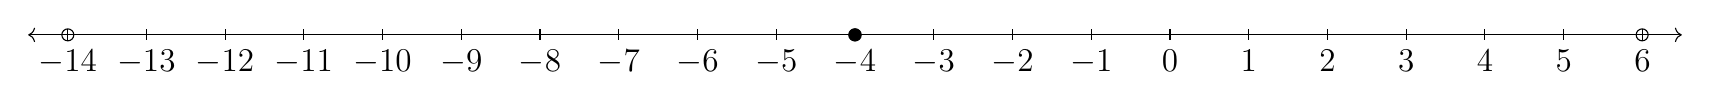
\begin{tikzpicture}
  \tkzInit[xmax=7,ymax=10,xmin=-15,ymin=-2]
\draw[<->] (-14.5,0) -- (6.5,0) ; %edit here for the axis
\foreach \x in {-14,-13,...,5,6} % edit here for the vertical lines
  \draw[shift={(\x,0)},color=black] (0pt,2pt) -- (0pt,-2pt);
\foreach \x in {-14,-13,...,5,6} % edit here for the numbers
  \draw[shift={(\x,0)},color=black] (0pt,0pt) -- (0pt,-2pt) node[below] {\large$\x$};
\draw[*-o] (-4.08,0) -- (6.08,0);
\draw[o-*] (-14.08,0) -- (-3.92,0);
%\draw[very thick] (0.92,0) -- (1.92,0);
\end{tikzpicture}
\end{document}
